\documentclass[border=3pt]{standalone}
% Preâmbulo compartilhado pelos diagramas TikZ da aula
\usepackage[T1]{fontenc}
\usepackage[utf8]{inputenc}
\usepackage{lmodern}
\usepackage{amsmath}
\usepackage{xcolor}
\usepackage{tikz}
\usetikzlibrary{arrows.meta,angles,quotes,decorations.pathmorphing,calc,
                positioning,shapes.geometric,backgrounds,fit}

% Paleta (mesma dos SVGs originais)
\definecolor{dblue}{HTML}{2A5B8C}
\definecolor{dorange}{HTML}{B3541E}
\definecolor{dgreen}{HTML}{4A7C59}
\definecolor{dred}{HTML}{9C4B4B}
\definecolor{dcream}{HTML}{F4F1EA}
\definecolor{dshade}{HTML}{DDD7C9}

% Estilos comuns (prefixo d... para não colidir com chaves internas do pgf)
\tikzset{
  >={Stealth[length=2mm]},
  dguide/.style={gray!55, dashed, line width=0.4pt},
  daxis/.style={gray!60, line width=0.7pt, ->},
  dbody/.style={fill=black!3, draw=black!80, line width=1pt},
  dacc/.style={draw=dblue, line width=1pt},
  dlbl/.style={black!55, font=\small},
  dsub/.style={black!45, font=\footnotesize},
  dstate/.style={circle, draw=black!80, fill=dcream, line width=1pt,
                 minimum size=17mm, font=\large, inner sep=1pt},
  dobs/.style={circle, draw=black!80, fill=dshade, line width=1pt,
               minimum size=14mm, font=\large, inner sep=1pt},
  dbox/.style={rounded corners=2pt, draw=black!80, fill=dcream, line width=1pt,
               align=center, inner sep=6pt},
  dtrans/.style={->, dblue, line width=1pt},
  dmeas/.style={->, dorange, line width=1pt},
}

\begin{document}
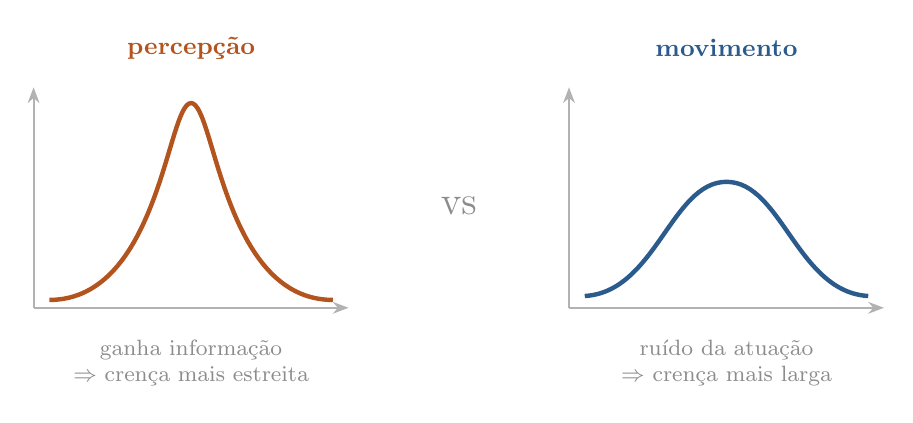
\begin{tikzpicture}[x=1cm,y=1cm]

  % --- percepção: crença estreita (mais certeza) ---
  \begin{scope}
    \node[dorange, font=\small\bfseries] at (2,3.3) {percepção};
    \draw[daxis] (0,0) -- (4,0);
    \draw[daxis] (0,0) -- (0,2.8);
    \draw[dorange, line width=1.6pt]
      (0.2,0.1) .. controls (1.6,0.1) and (1.7,2.6) .. (2.0,2.6)
                .. controls (2.3,2.6) and (2.4,0.1) .. (3.8,0.1);
    \node[dsub, align=center] at (2,-0.7) {ganha informação\\$\Rightarrow$ crença mais estreita};
  \end{scope}

  % seta
  \node[black!45, font=\Large] at (5.4,1.3) {vs};

  % --- movimento: crença larga (menos certeza) ---
  \begin{scope}[shift={(6.8,0)}]
    \node[dblue, font=\small\bfseries] at (2,3.3) {movimento};
    \draw[daxis] (0,0) -- (4,0);
    \draw[daxis] (0,0) -- (0,2.8);
    \draw[dblue, line width=1.6pt]
      (0.2,0.15) .. controls (1.1,0.2) and (1.3,1.6) .. (2.0,1.6)
                 .. controls (2.7,1.6) and (2.9,0.2) .. (3.8,0.15);
    \node[dsub, align=center] at (2,-0.7) {ruído da atuação\\$\Rightarrow$ crença mais larga};
  \end{scope}

\end{tikzpicture}
\end{document}
